\documentclass[12pt,a4paper,twoside]{report}

\usepackage{fancyhdr}
\usepackage{lastpage}
\usepackage{a4wide} 
\usepackage{amsmath}
\usepackage{amssymb} 
\usepackage{graphicx}
\usepackage{color}
\usepackage{fancybox}
%\usepackage{moreverb}
\usepackage[T1]{fontenc}
% \usepackage{hangcaption}
\usepackage{hyperref}
\usepackage{listings}
\usepackage[latin9]{inputenc}
\usepackage[francais]{babel}
\frenchbsetup{StandardItemLabels}

%\fbox{}
%\shadowbox{}
%\doublebox{}
%\ovalbox{}
%\Ovalbox{}
%\shabox{}


% --- Logo Atos ---
%\makebox[\textwidth][l]{
%\raisebox{-15pt}[0pt][0pt]{
%\hspace{2.5cm}
%\includegraphics[scale=0.1]{Images/logo_atos.eps}
%}
%}
\title{Rapport de projet de fin d'\'etudes}
\author{Nom et Prénom Etudiant}
\date{\today}

\pagestyle{headings}

\begin{document}
%\lstset{ numbers=left, tabsize=3, frame=single, numberstyle=\ttfamily, basicstyle=\footnotesize} 
\thispagestyle{empty}

\begin{center}
\makebox[\textwidth][l]{
\raisebox{-8pt}[0pt][0pt]{
%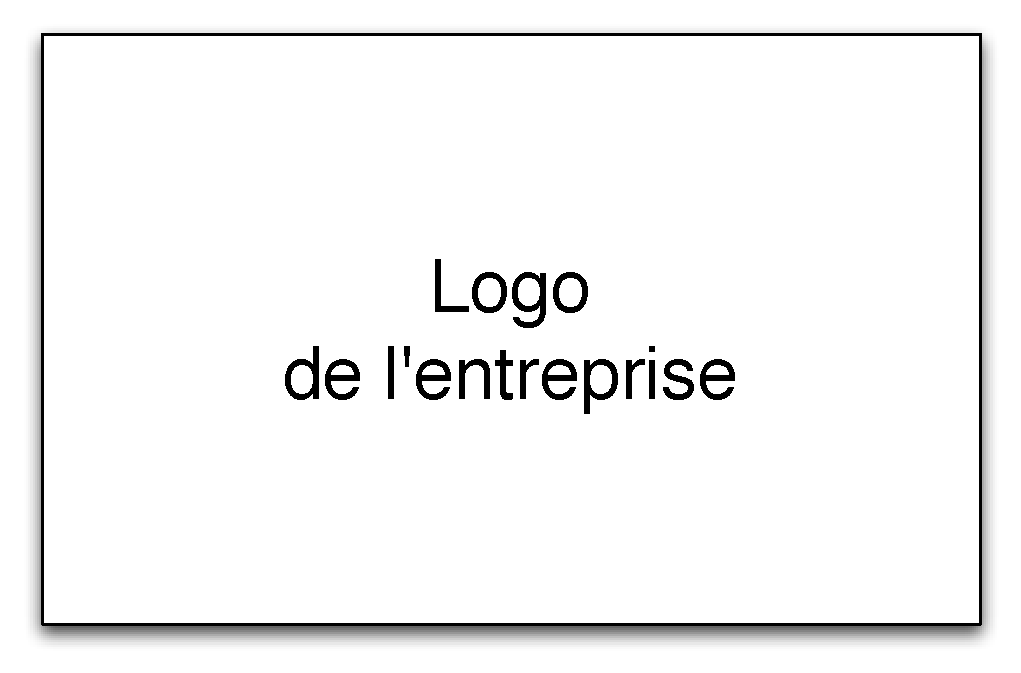
\includegraphics[scale=0.18]{Images/logo_entreprise}
}
}
\makebox[\textwidth][r]{
\raisebox{0pt}[0pt][0pt]{

\includegraphics[scale=0.2]{Images/logo_ensimag.PNG}
}
}
Grenoble INP  -- ENSIMAG\\
Ecole Nationale Sup\`erieure d'Informatique et de Math\'ematiques Appliqu\'ees\\
\vspace{3cm}
{\LARGE Rapport de Projet de Fin d'Etudes }\\
\vspace{1cm}
Effectu\'e chez Amundi en tant que prestataire Aubay\\
\vspace{2cm}
\shadowbox{
\begin{minipage}{1\textwidth}
\begin{center}
{\Huge Titre du Sujet de Stage}\\
\end{center}
\end{minipage}
}\\
\vspace{3cm}
Andr\'e Mathilde\\
3A -- Graphics, Vision and Robotics\\
\vspace{3mm}
02 Mars 2015 -- 31 Ao\^ut 2015\\
\vspace{3,5cm}
\begin{tabular}{p{10cm}p{10cm}}
{\bf Amundi}                                            &{\bf Responsable de stage}\\
{\footnotesize 90 Boulevard Pasteur}       & ~~~Nom Et Prenom Tuteur Entreprise\\
{\footnotesize BP XX}                                        & {\bf Tuteur de l'ecole}\\
{\footnotesize 75015 Paris}                          & ~~~Rippert Christophe\\
\end{tabular}
\end{center}
\newpage
\renewcommand{\contentsname}{Table des mati\`eres} % Dans le corps du document,avant la commande \tableofcontents.
\tableofcontents

\newpage
\chapter{R�sum�}
En derni�re ann�e de cycle ing�nieur � l'ensimag Grenoble, les �tudiants sont amen�s � effectuer un 
stage en entreprise d'une dur�e de six mois. \\

Jai effectu� mon stage de Mars � Aout 2015 pour la Soci�t� de Service en Ing�nierie Informatique (SSII) AUBAY, en mission chez leur client AMUNDI.\\

J'ai �t� amen�e � travailler autour d'un logiciel interne � AMUNDI, nomm� AMEX pour Amundi Exchange Message. 
J'ai fait parti de l'�quipe MFN (Middle Flux N�gociation) qui regroupe une vingtaine de personnes et dont le responsable est Jean-Fran�ois Morin. Cette �quipe g�re plusieurs applications dont la plateforme internationale Amundi Exchange Message, Amex qui permet de transmettre des messages intra applicatifs et inter banques suivant des formats standards entre les diff�rents partenaires. Ce projet est principalement pris en charge par Pierre Chatelier, qui m'a suivi et encadr� tout au long de ma mission. 




\chapter{Introduction}

Mon stage se d�roule actuellement chez Amundi, dans l'�quipe Middle Flux (MFX), pour la soci�t� de service Aubay. Ce document pr�sente l'avancement du projet de fin d'�tude apr�s six semaines de travail dans l'entreprise. \\






Au cours de ce rapport, je vais tout d'abord vous pr�senter AUBAY l'entreprise m'ayant fourni ce stage ainsi que son client Amundi chez qui j'ai travaill�. Dans un second temps, les probl�matiques et objectifs du projet au sein de l'entreprise seront d�velopp�s, vous pourrez ainsi lire une description du logiciel sur lequel j'ai travaill�. Je vous d�crirai ensuite les solutions techniques et l'avancement de mon projet apr�s six semaines de stage, pour finir avec mes impressions personnelles.   


\newpage
\chapter{Pr�sentation des entreprises}

\section{Aubay}

\section{Amundi}
Amundi est une soci�t� de conseil en �pargne salariale, n�e du partenariat du groupe Cr�dit Agricole SA (actionnaire � 80\%) et de la Soci�t� G�n�rale (actionnaire � 20\%). 
Cette entreprise de gestion des actifs compte parmis les plus grands acteurs de l'industrie de l'asset management
mondial.

Un Asset Manager cr�e et g�re au quotidien des produits de placements, � savoir les OPCVM (Organisme de Placement Commun en Valeurs Mobili�res). Les particuliers et les entreprises souhaitant confier leur argent pour qu'il soit g�r� peuvent faire appel � un Asset Manager. 



\section{Mon stage au sein de l'entreprise}
Dans le cadre de mon projet de fin d'�tude, j'ai int�gr� le service informatique d'Amundi et plus pr�cis�ment l'�quipe MFX, pour Middle Flux, dirrig�e par Jean-Fran�ois Morin.

Le domaine MFX a en charge le d�veloppement et la maintenance des applications utilis�es par le Middle Office Flux Amundi. Celui-ci se d�compose en deux �quipes, la maitrise d'ouvrage (MOA) et la maitrise d'Oeuvre (MOE). Je fais partie de cette derni�re. \\

Dans le domaine on va distinguer quatre types d'applications : 
\begin{enumerate}
	\item Applications permettant d'assurer le cycle de vie des transactions : ETC (Electronic Trade Confirmation) pour le Matching Broker et ETD (Electronic Trade Delivery) pour le r�glement-livraison (le d�positaire et le valorisateur).
	\item Application permettant d'assurer le cycle de vie des titres financiers (Int�gration des op�rations sur titres) : MOCA, Middle Office Corporate Action.
	\item Application permettant l'int�gration des collectes des souscription-rachats sur les fonds Amundi : GSR, Gestion des souscriptions-rachats.
	\item Une plateforme d'�change AMEX dont le p�rim�tre va au del� du domaine MFX, mais dont le d�veloppement et la maintenance du socle technique est de la responsabilit� du domaine MFX. 
\end{enumerate}


Amundi g�re certaines applications qui ont besoin de communiquer entre elles en envoyant et re�evant de nombreux messages. Ces derniers transitent � travers une m�me application appel�e Amex. 
J'ai travaill� sur la plateforme Amex et plus pr�cis�ment sur une refonte totale d'un de ses composants, les FlowDetails. Le but principal de cette refonte pour les �quipes utilisant AMEX est une am�lioration des performances.\\ 

\begin{figure}[!h] %on ouvre l'environnement figure
\center
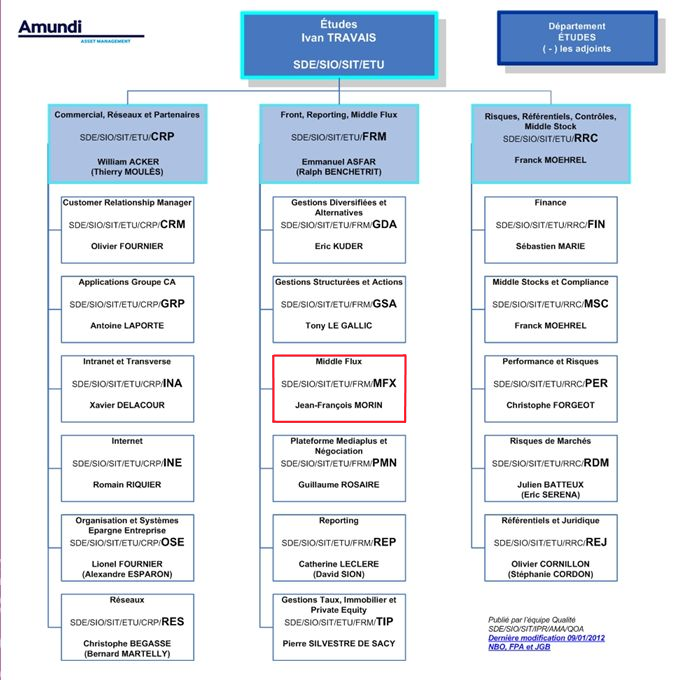
\includegraphics[scale=0.5]{Images/organigrammeEquipes.png}
\caption{Organigramme de Amundi IT Services} %la l�gende
\end{figure} %on ferme l'environnement figure




\newpage
\chapter{Probl�matique et objectifs}

\section{Contexte du projet}
\subsection{Le cadre : AMEX}
L'application AMEX est une plateforme d'�change de messages pouvant g�rer aussi bien des �changes inter-applicatifs au sein du syst�me d'information que des �changes avec des applications externes de partenaires d'Amundi.
C'est une plateforme multi-format et multi-canal. Elle permet l'�change de messages sous diff�rents formats, ceux-ci pouvant �tre standaris�s; (le plus connu est SWIFT, format cr�� par un partenariat des plus grandes banques mondiales) ou propri�taires c'est � dire d�velopp� spr�cialement pour communiquer avec un partenaire sp�cifique. Les messages peuvent �tre envoy�s via diff�rents supports (JMS, Web Services, Fax, Fichier, File MQ, Imprimantes, Mail). \\



\begin{figure}[ht!] %on ouvre l'environnement figure
\centering
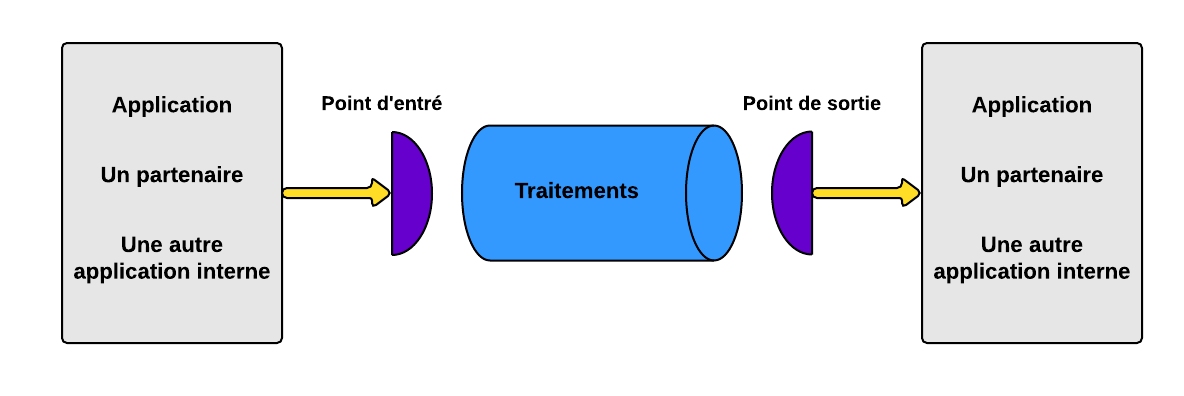
\includegraphics[scale=0.8]{Images/amex.png}
\caption{Les flux Amex} %la l�gende
\end{figure} %on ferme l'environnement figure

Amex regroupe une centaine de flux. Ils sont utilis�s notament pour la conversion d'un message d'un format X vers un format Y. 
Cela peut se faire via un format d'�change pivot : le STPML qui est cr�� � partir du XML. 
\\
Il �xiste diff�rentes API dans Amex utilisant les FlowDetails. 
Le service d'audit a pour but de tracer tous les messages transitant par Amex. L'audit se fait dans des tables en base de donn�es. Il �xiste diff�rents statuts d'Audit d�crivant le statut du message transitant, par exemple un message a comme statut PENDING � sa g�n�ration, SENT � son envoi si un acquittement est attendu, SENT NO\_ACK � son envoi si aucun acquittement n'est attendu, ACKNOWLEDGED � son acquittement, ERROR en cas d'erreur . \\

Il est possible de param�trer des taches automatiques � �x�cuter lorsqu'un message transitant par Amex passe dans un certain statut d'audit. C'est le role du service de taches automatiques. Celles-ci peuvent etre un envoi d'un mail, un appel � un web service distant ou le post d'un message sur une file JMS ou MQ. \\
\\
Un flowdetail est un composant technique d�crivant l'entr�e ou la sortie d'un flux de communication. Ainsi lors de la cr�ation d'un nouveau flux, l'utilisateur cr�e deux Flowdetails, un repr�sentant l'entr� du flux (input) et un autre repr�sentant sa sortie (output). Un flowdetail contient des informations permettant de connaitre l'emetteur et le destinataire du message ainsi que son format, m�dia (d'entr�e ou de sorti). 
Ce composant est n�cessaire pour le routage du message mais aussi pour l'audit. 
L'image ci-dessous montre les informations regroup�es dans un FlowDetails.

\begin{figure}[ht!] %on ouvre l'environnement figure
\centering
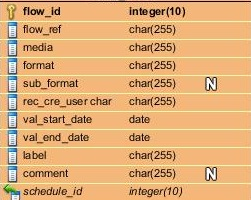
\includegraphics[scale=0.8]{Images/FlowDetails.jpg}
\caption{Un FlowDetails} %la l�gende
\end{figure} %on ferme l'environnement figure





\subsection{Utilisation des FlowDetails}
Un logiciel d�velopp� en interne chez Amundi appel� MediaPlus Alto propose un module permettant de g�rer les FlowDetails : les visualiser, les cr�er, les supprimer et les modifier. 
Mais d'autres modules utilisent aussi les FlowDetails � travers des arbres RuleSolver notament. Ces modules offrent la possibilit� d'�diter des arbres de r�gles et de les sauvegarder. Un arbre RuleSolver peut par exemple, servir � retourner la liste des t�ches � effectuer selon tel ou tel type. 

Ces modules sont utilis�s par des personnes de la MOE principalement pour des tests et par des personnes de la MOA lors de la cr�ation de nouveaux flux. Le but de mon stage est de faciliter le travail de ces personnes en proposant une impl�mentation plus efficace des FlowDetails. La premi�re image ci-dessous est la vue du logiciel, permettant de visualiser ou de cr�er des FlowDetails. 

\begin{figure}[ht!] %on ouvre l'environnement figure
\centering
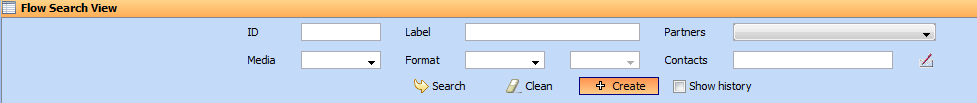
\includegraphics[scale=0.6]{Images/AltoFD.png}
\caption{Visualisation des FlowDetails} %la l�gende
\end{figure} %on ferme l'environnement figure

La seconde image est le r�sultat s'affichant apr�s avoir cliqu� sur le bouton 'Create' et choisi 'Mail' comme m�dia. L'utilisateur doit choisir un Format, plusieurs contacts mail (FROM, TO). Cliquer sur le bouton 'Save' cr�era le FlowDetail.

\begin{figure}[ht!] %on ouvre l'environnement figure
\centering
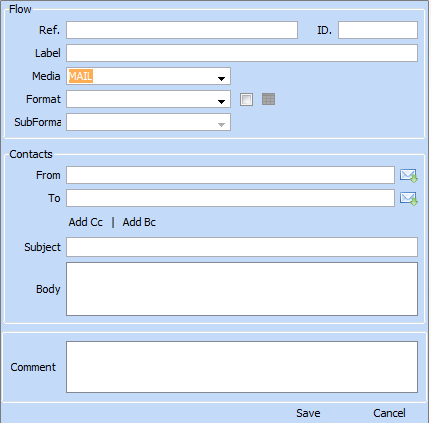
\includegraphics[scale=0.8]{Images/AltoCreate.png}
\caption{Creation d'un flowdetail Mail} %la l�gende
\end{figure} %on ferme l'environnement figure



\newpage
\section{Travail � r�aliser}
Mon stage de six mois consiste en une refonte totale du composant FlowDetails. Le but principal �tant d'am�liorer les performances notament lors de la cr�ation des FlowDetails mais aussi de permettre une mod�lisation plus claire et �volutive. Lors de la cr�ation d'un FlowDetail � partir de l'interface, les �tapes sont tr�s lentes, avant qu'une fen�tre s'affiche pour la premi�re fois, il faut souvent attendre plusieurs secondes, ce qui rend le travail de certaines personnes nettement moins efficace. 
Le premier d�veloppement d'Amex a �t� r�alis� il y a ... ans. Les besoins et la quantit� de flux et de messages �chang�s
ont beaucoup augment� depuis. Par exemple, des informations sur des contacts sont enregistr�s dans une base de donn�es.
Ces informations ont �volu�s au fil du temps, par exemple si un message de format SWIFT transite dans AMEX, deux 
informations sont n�cessaires : le BIC du contact ainsi que son DN distinguish name. La mod�lisation de d�part n'�tant pas tr�s g�n�rique un deuxi�me attribut a donc �t� ajout� pour tous types de contacts (Mail, Jms, Printer, SWIFT...), mais celui-ci a une valeur nul pour tous les autres que SWIFT. Ceci �tait un probl�me a r�soudre, et ainsi de rendre la mod�lisation
plus �volutives pour d'�ventuels changements futurs. 
\\
Afin d'effectuer une refonte de ce composant, mon travail a �t� divis� en trois principales �tapes. 

La premi�re �tape a �t� d'analyser l'�xistant afin de comprendre la mod�lisation actuelle des FlowDetails et les diff�rents services utilisant ce composant. Le but est ensuite de proposer une nouvelle mod�lisation base de donn�es de ces composants. 
Dans un deuxi�me temps, il faudra impl�menter et mettre en place la nouvelle mod�lisation et ainsi adapter les interfaces  Homme Machine (IHM). Le client d'administration des FlowDetails devra r�pondre aux besoins des MOA. 
La derni�re �tape consiste en l'exposition de ces services d'administration sous forme de service REST afin de permettre un d�couplage applicatif n�cessaire aux �volutions du middleware.  
\\
Le diagramme de Gantt ci dessous pr�sentes les diff�rentes �tapes. Voir en annexe pour 
connaitre les dates d'�ch�ance qui ont �t� fix�es en d�but de stage.
\begin{figure}[ht!] %on ouvre l'environnement figure
\centering
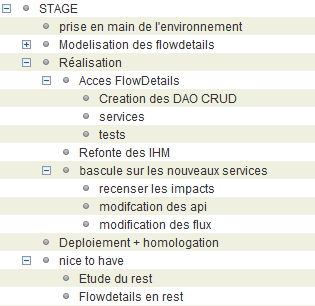
\includegraphics[scale=0.9]{Images/gantt1.png}
\caption{Diagramme de Gantt} %la l�gende
\end{figure} %on ferme l'environnement figure

Mon travail a �t� r�alis� suivant un cycle pr�cis permettant d'aboutir � une validation de chacune des �tapes.

\begin{figure}[ht!] %on ouvre l'environnement figure
\centering
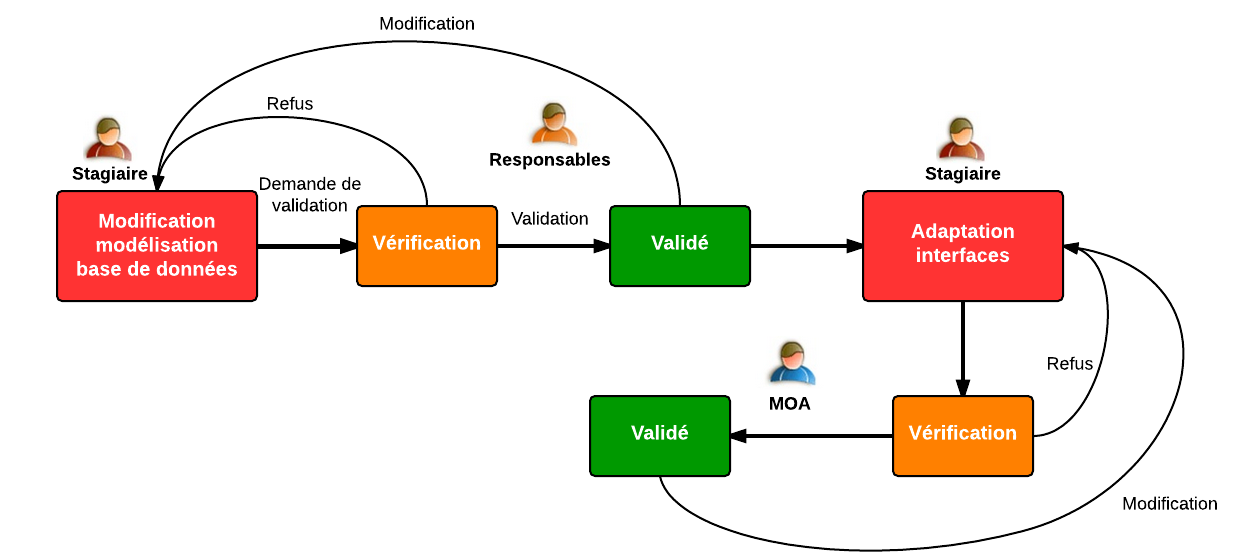
\includegraphics[scale=0.8]{Images/workflow.png}
\caption{Worflow du projet} %la l�gende
\end{figure} %on ferme l'environnement figure


\section{Objectifs pr�cis}



\newpage
\chapter{Les solutions techniques}

\section{Synth�se de l'existant}
Avant de vous d�crire la partie technique de mon travail, je vais vous introduire les principales technologies et principaux logiciels que j'ai utilis�. \\

\subsection{Langage de d�veloppement}
L'application sur laquelle je travaille est d�velopp� en Java EE, soit Java Entreprise Edition. C'est la version de Java destin�e aux applications des entreprises. 

\subsection{Les outils utilis�s}

\subsection{Les termes techniques}

\section{Description du travail}

\subsection{Analyse de l'�xistant}
La premi�re phase de mon travail a consist� en une analyse de la mod�lisation base de donn�es des FlowDetails. Apr�s avoir install� l'environnement de travail et tous les outils n�cessaires, j'ai pu analyser le projet et plus particuli�rement tout ce qui concernait les FlowDetails. \\

Ainsi, j'ai pu r�aliser un diagramme entit� relations repr�sentant la mod�lisation base de donn�es des FlowDetails. Voir annexe : Mod�lisation des FlowDetails existants. Cela m'a permis d'analyser tous les objets en relation avec les FlowDetails.  

\subsubsection{Les API utilisant les FlowDetails}
Dans la plateforme Amex, il y a diff�rentes services  qui utilisent les flowdetails. Je vais d�crire le fonctionnement de chacun d'eux. \\

Le service d'audit a pour but de tracer tous les messages transitant par Amex. L'audit se fait dans des tables en base de donn�es. Il �xiste diff�rents statuts d'Audit d�crivant le statut du message transitant, par exemple un message a comme statut PENDING � sa g�n�ration, SENT � son envoi si un acquittement est attendu, SENT NO\_ACK � son envoi si aucun acquittement est attendu, ACKNOWLEDGED � son acquittement, ERROR en cas d'erreur . \\

Il est possible de param�trer des taches automatiques � �x�cuter lorsqu'un message transitant par Amex passe dans un certain statut d'audit. C'est le role du service de taches automatiques. Ces taches automatiques peuvent etre un envoi d'un mail, un appel � un web service distant ou le post d'un message sur une file JMS ou MQ.
Il �xiste des objets TaskHandler permettant de savoir comment cr�er le message � envoyer et � qui l'envoyer. Ces informations sont contenues dans la table TaskHandler et sont param�trables via des arbres RuleSolver. 



\subsection{La nouvelle mod�lisation}

\subsection{Migration de l'existant}

\section{Protocole d'�valuation}


\newpage

\chapter{Avancement du projet}


\newpage
\chapter{Impressions personnelles}

\newpage
\chapter{annexe}

\section{Lexique}

\textbf{Flux}
Un flux permet l'envoi et la reception de données. Ils traitent les données de manière séquentielle ou asynchrones.



\textbf{Swift}


\begin{figure} %on ouvre l'environnement figure
\centering
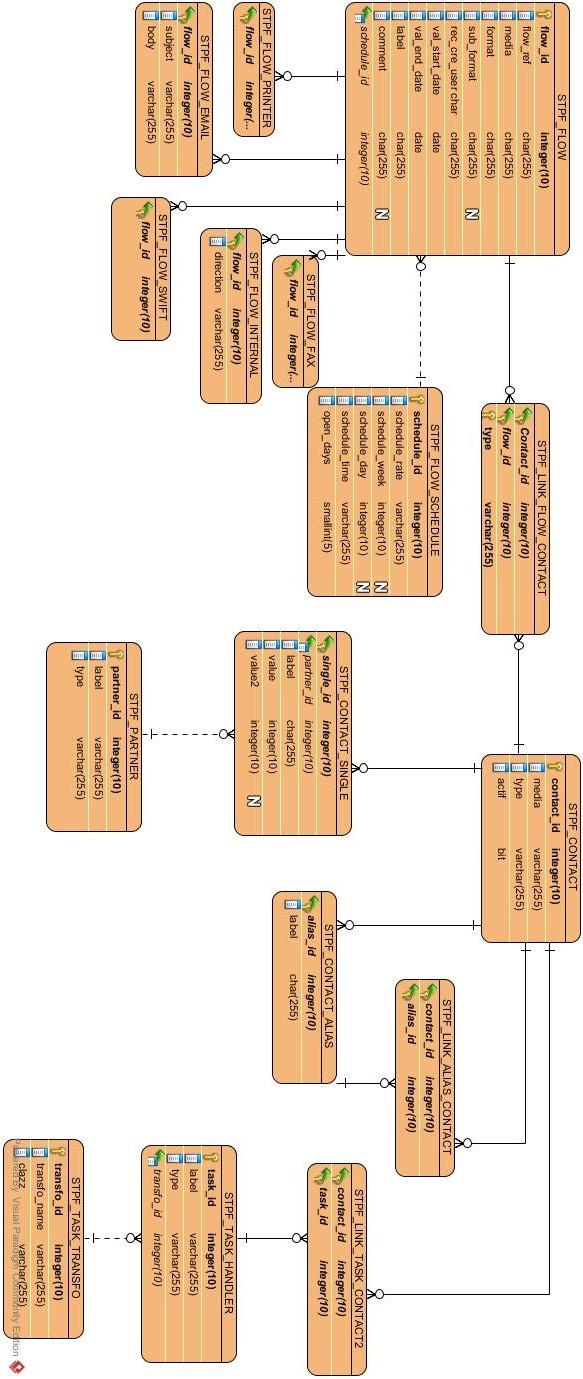
\includegraphics[scale=0.6]{Images/FlowDetailsExistant.jpg}
\caption{Diagramme entité relation de la modélisation existante} %la légende
\end{figure} %on ferme l'environnement figure

\newpage
\begin{figure} %on ouvre l'environnement figure
\centering
\includegraphics[width=14cm, height=23cm]{Images/Gantt.png}
\caption{Diagramme de Gantt} %la légende
\end{figure} %on ferme l'environnement figure
\end{document}
